\documentclass[12pt]{article}
\usepackage[utf8]{inputenc}
\usepackage[T1]{fontenc}
\usepackage{geometry}
\usepackage{graphicx}
\usepackage{makeidx}
\geometry{margin=2.5cm}

\title{Informe - Práctica \#1}
\author{Tu nombre}
\date{Fecha de entrega}

\begin{document}
	
	\thispagestyle{empty}
	
	\begin{center}
		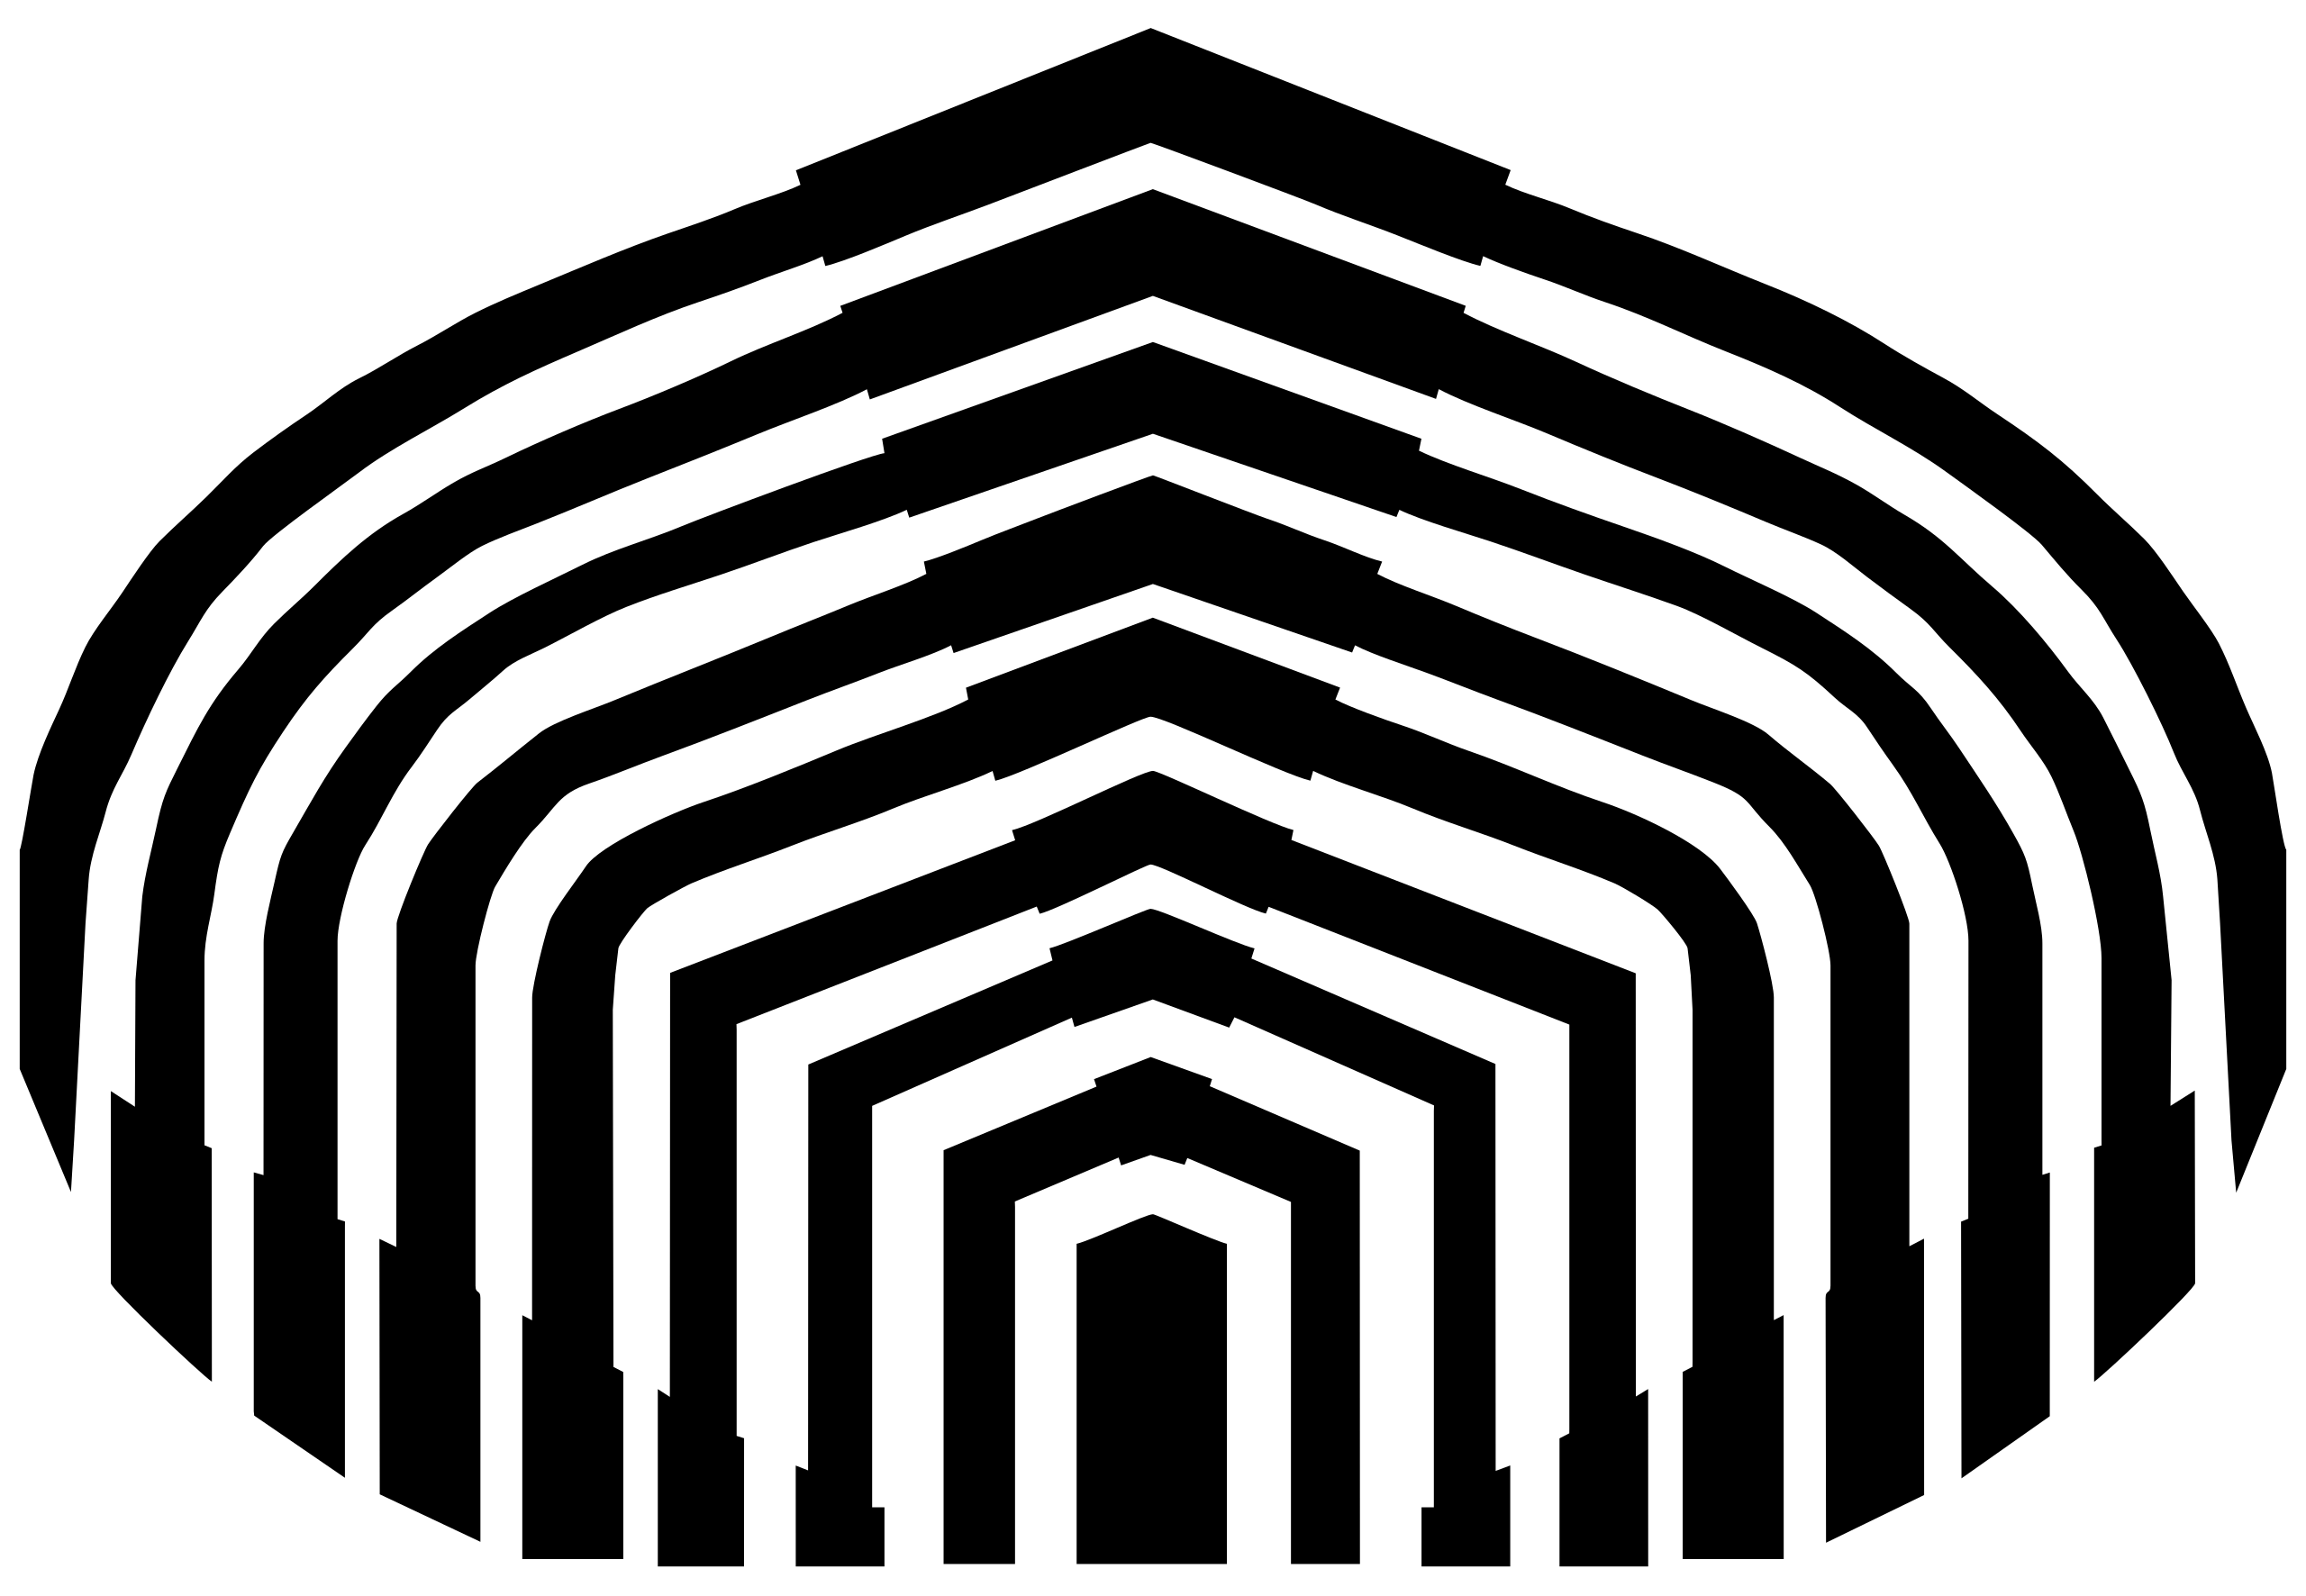
\includegraphics[width=3.1cm,height=2cm]{logo}\\
		UNIVERSIDAD SIMÓN BOLÍVAR\\
		DEPARTAMENTO DE ELECTRÓNICA Y CIRCUITOS\\
		EC1281 - LABORATORIO DE MEDICIONES ELÉCTRICAS\\
		SECCIÓN 1 - GRUPO 1\\
		
		\vspace{7cm}
		\textbf{\Large INFORME - PRÁCTICA \#}\\
		INTRODUCCIÓN AL LABORATORIO\\
	\end{center}
	
	\begin{flushleft}
		\vspace{9cm}
		\hfill Integrantes:\\
		\hfill {\large Luis Becerra - 1910557}\\
		\hfill {\large Lorena Rojas - 1910469}\\
	\end{flushleft}
	
	\newpage
	
	\pagenumbering{roman}
	
	\begin{center}
		\textbf{\large RESUMEN}\\
	\end{center}
	
	Inserte resumen
	
	\newpage
	
	\begin{center}
		\textbf{\large ÍNDICE}\\
	\end{center}
	
	\noindent \textbf{RESUMEN} \hfill \textbf{I}\\
	\noindent \textbf{ÍNDICE} \hfill \textbf{II}\\
	\noindent \textbf{MARCO TEÓRICO} \hfill \textbf{1}\\
	\noindent \textbf{METEODOLOGÍA} \hfill \textbf{4}\\
	\noindent \textbf{RESULTADOS} \hfill \textbf{5}\\
	\noindent \textbf{ANÁLISIS DE RESULTADOS} \hfill \textbf{13}\\
	\noindent \textbf{CONCLUSIONES} \hfill \textbf{14}\\
	\noindent \textbf{COMENTARIOS FINALES} \hfill \textbf{15}\\
	
	\newpage
	
	\pagenumbering{arabic}
	
	\begin{center}
		\textbf{\large MARCO TEÓRICO}\\
	\end{center}
	
	\textbf{1. }\\
	
	Inserte inciso 1
	
	\begin{itemize}
		\item \textbf{Sub-elemento 1 del inciso } inserte lo que corresponda
		
	\end{itemize}
	
	\newpage
	
	\begin{center}
		\textbf{\large RESULTADOS}\\
	\end{center}
	

	En esta parte se mostrarán las imágenes obtenidas en cada uno de los análisis circuitales en Spice.\\
	
	\begin{itemize}
		\item \textbf{Circuito 1}- Corresponde a la figura 2.1.a\\ 
		
		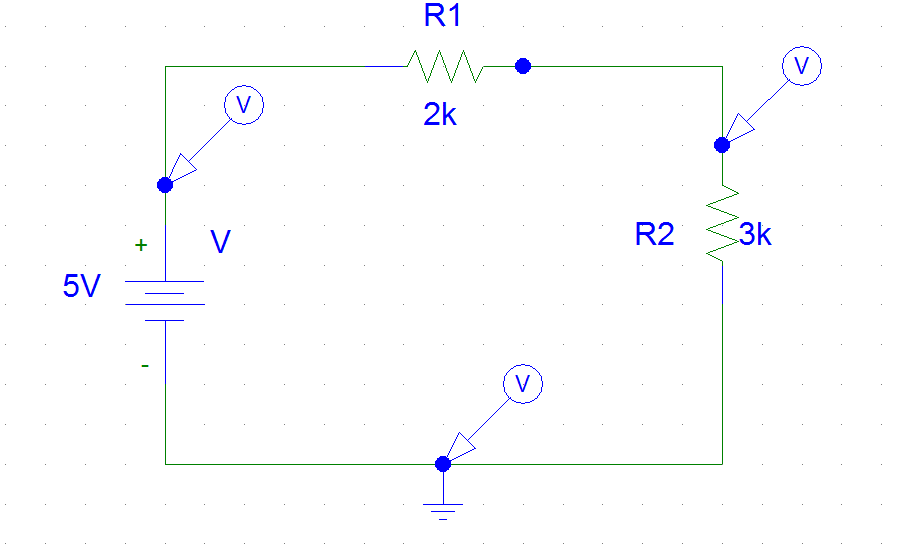
\includegraphics[width=11cm,height=7cm]{Img/dc_dos_resis.png}\\
		
		\noindent A este circuito se le realizaron los análisis transient y bias point detail obteniendo las siguientes gráficas de salida.\\
		
		\noindent En el análisis transient:\\
		
		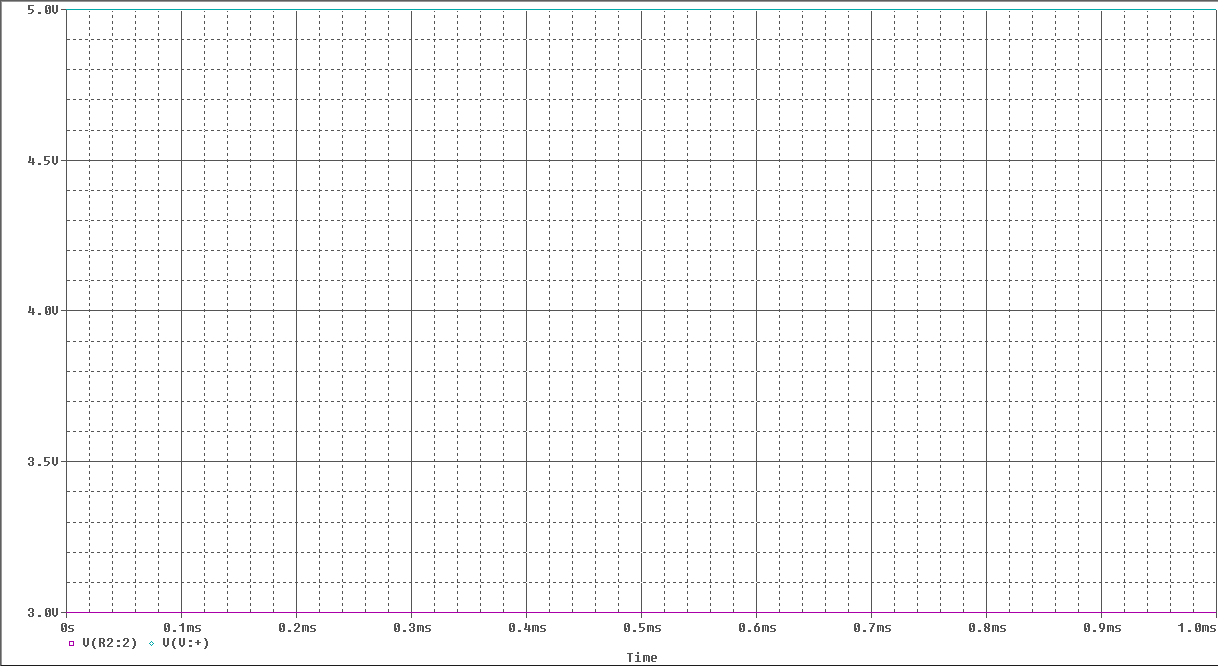
\includegraphics[width=11cm,height=7cm]{Img/Fuente_DC_y_dos_resistencias.png}
		
		\newpage
		 
		\noindent Y en el análisis bias point detail, se obtuvo:\\
		
		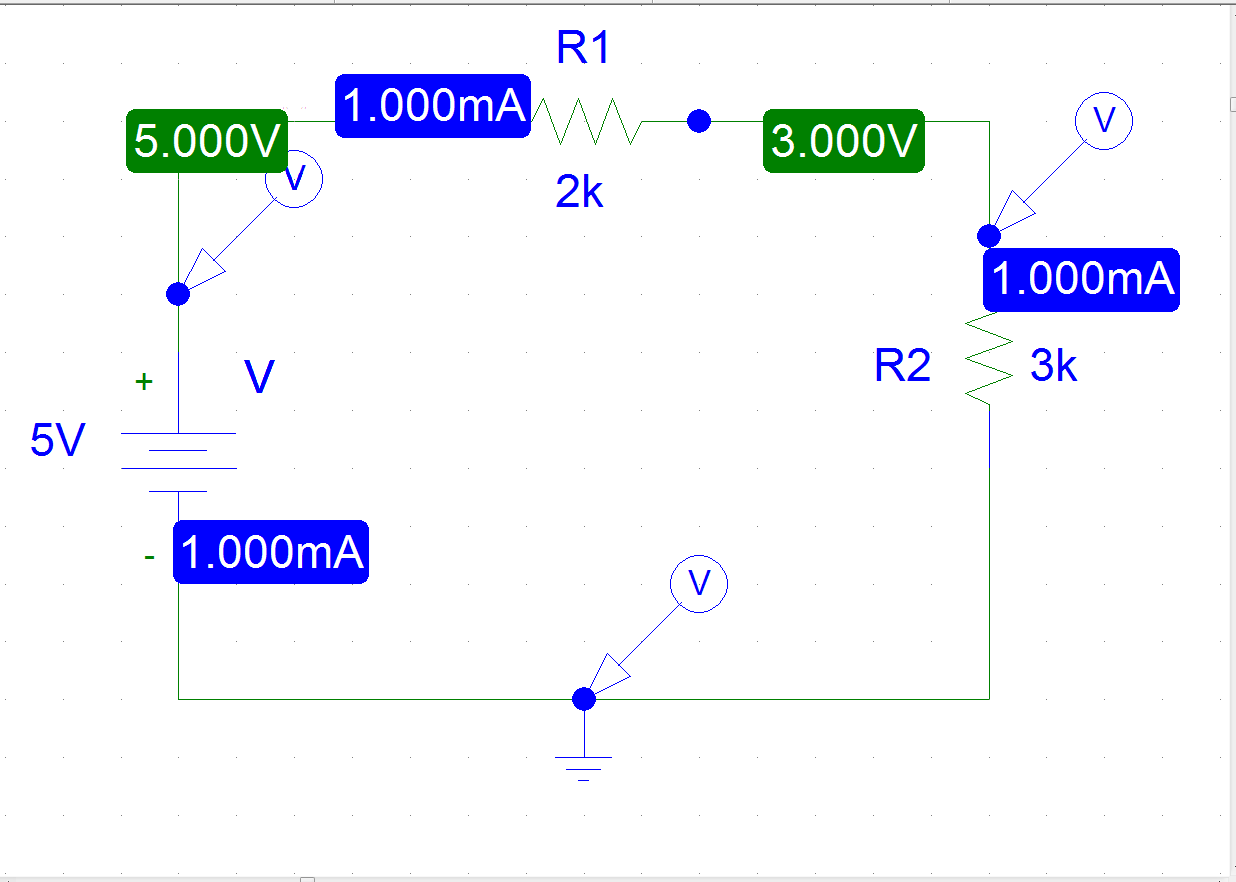
\includegraphics[width=11cm,height=7cm]{Img/Fuente_DC_y_dos_resistencias_Bias_analisis.png}\\
		
		\item \textbf{Circuito 2}- Corresponde a la figura 2.1.b\\ 
		
		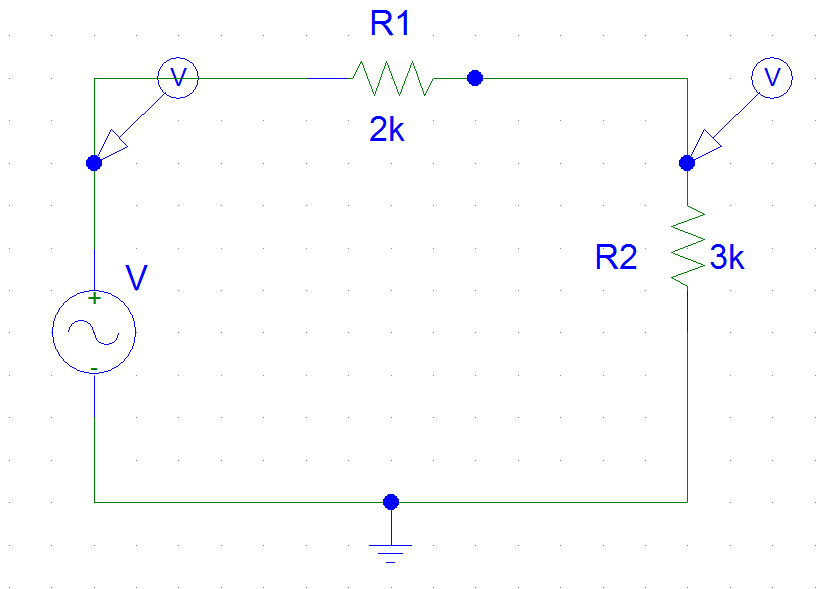
\includegraphics[width=11cm,height=7cm]{Img/ac_dos_resis.png}\\
		
		\noindent En este circuito sólo se aplicó el análisis transient, de donde se obtuvo:\\
		
		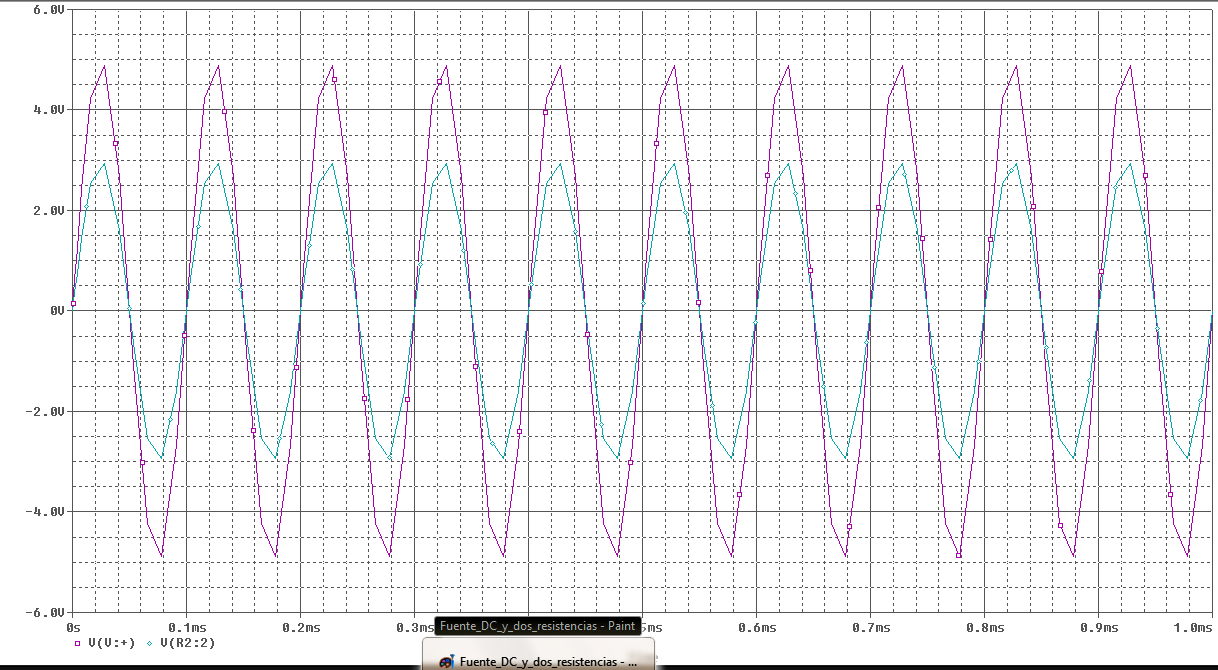
\includegraphics[width=11cm,height=7cm]{Img/Fuente_AC_y_dos_resistencias.png}\\
		
		\item \textbf{Circuito 3}- Corresponde a la figura 2.2.a\\ 
		
		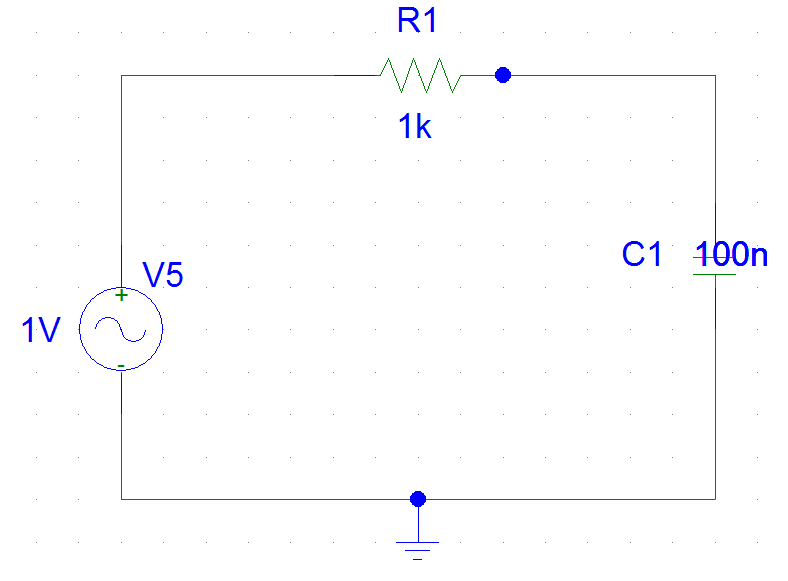
\includegraphics[width=11cm,height=7cm]{Img/ac_rc.png}\\
		
		\noindent Sobre este circuito se realizó un análisis transient, un análisis ac sweep y otro ac sweep sustituyendo la fuente por una de onda cuadrada.
		
		\noindent Transient\\
		
		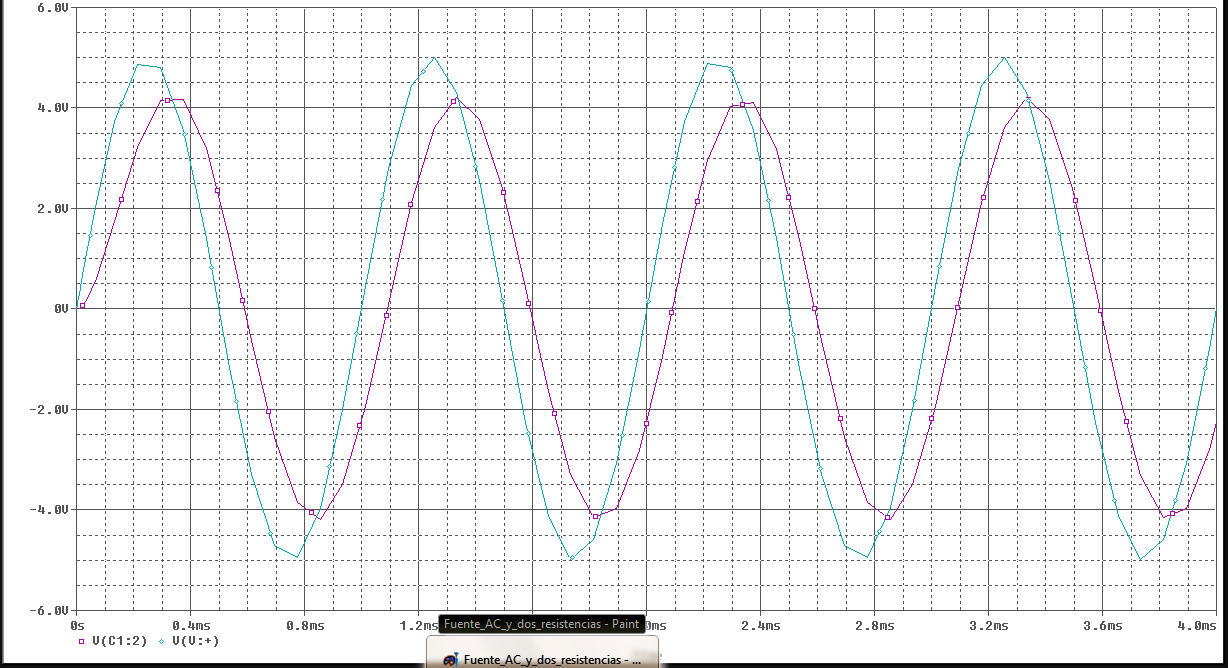
\includegraphics[width=11cm,height=7cm]{Img/Fuente_AC_RC.png}\\
		
		\noindent AC Sweep\\
		
		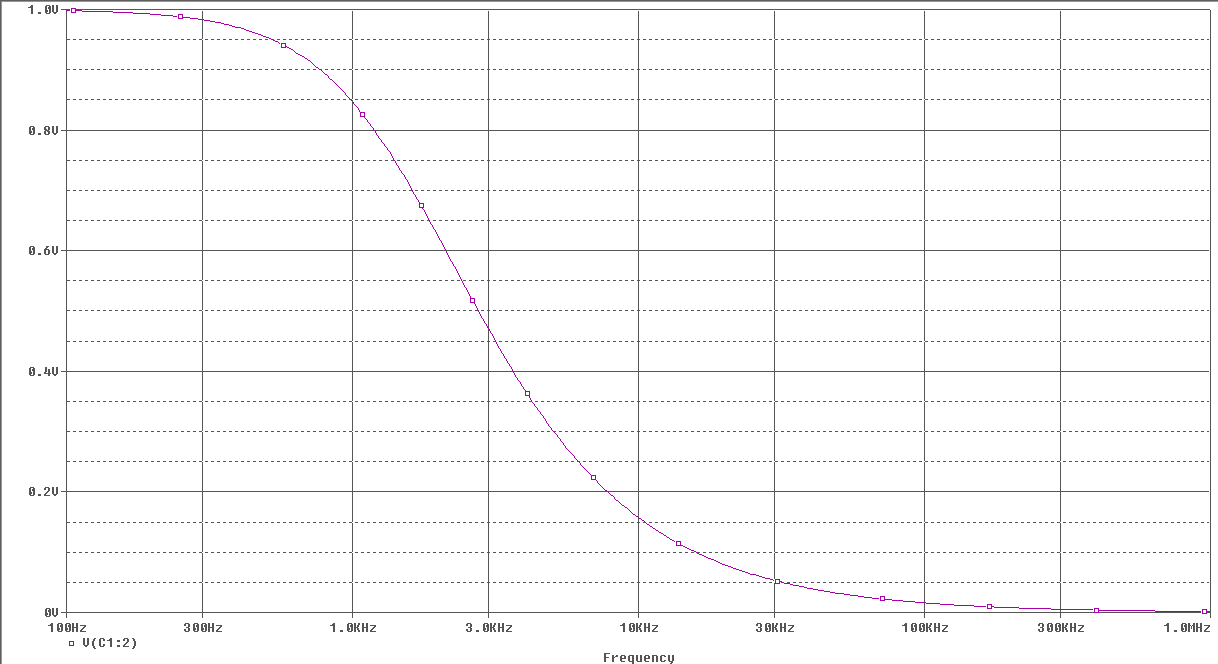
\includegraphics[width=11cm,height=7cm]{Img/Fuente_AC_RC_AC_sweep.png}\\
		
		\newpage 
		
		\noindent AC Sweep Vpulse\\
		
		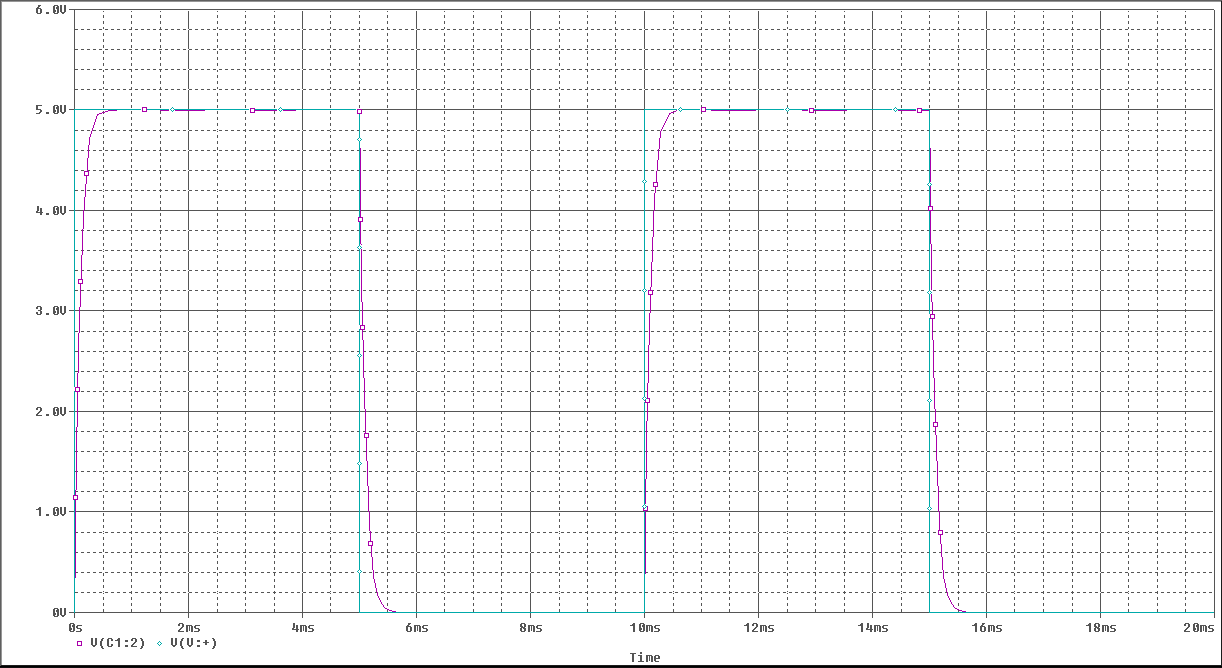
\includegraphics[width=11cm,height=7cm]{Img/Fuente_AC_RC_Vpulse}\\
		
		\item \textbf{Circuito 4}- Corresponde a la figura 2.2.b\\ 
		
		\noindent Es $L_2 = 100mH$ pero se nos pasó acomodar el display.\\
		
		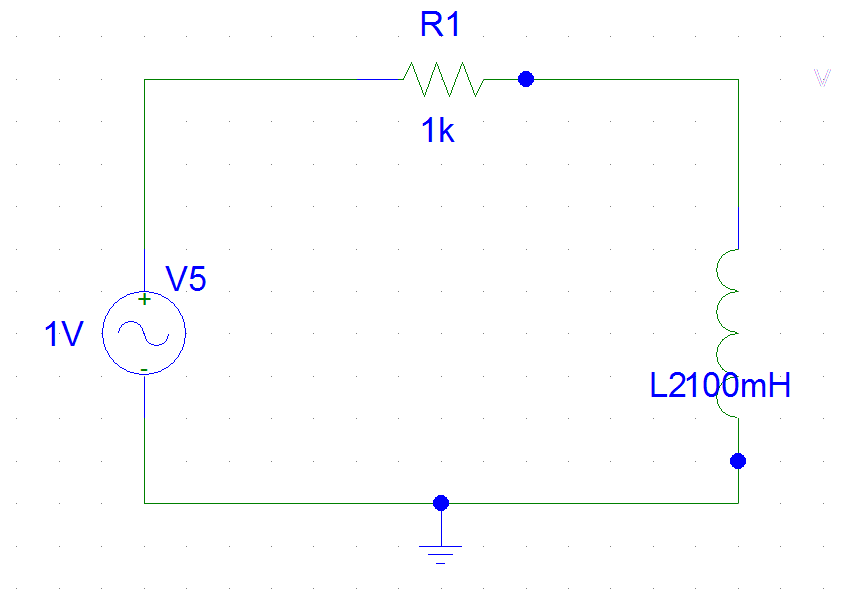
\includegraphics[width=11cm,height=7cm]{Img/ac_rl}\\
		
		\noindent Para este circuito también se hicieron los análisis transient, ac sweep y otro ac sweep con una fuente de onda cuadrada, quedando:
		
		\newpage
		
		\noindent Transient\\
		
		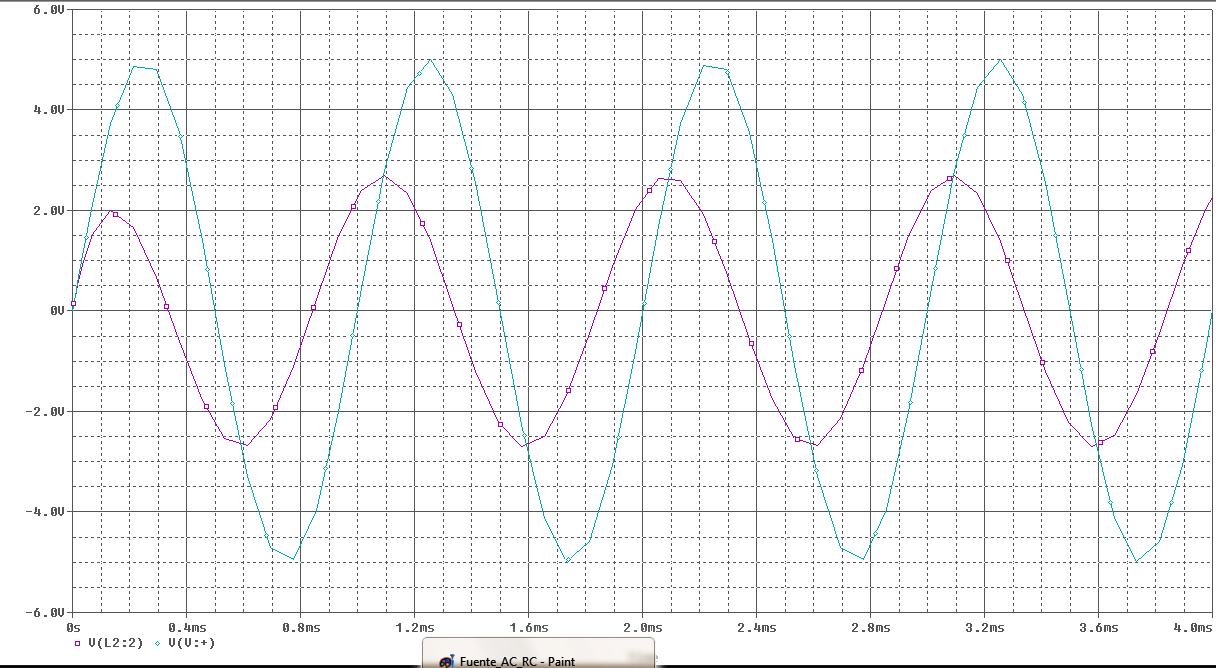
\includegraphics[width=11cm,height=7cm]{Img/Fuente_AC_RL}
		
		\noindent AC Sweep\\
		
		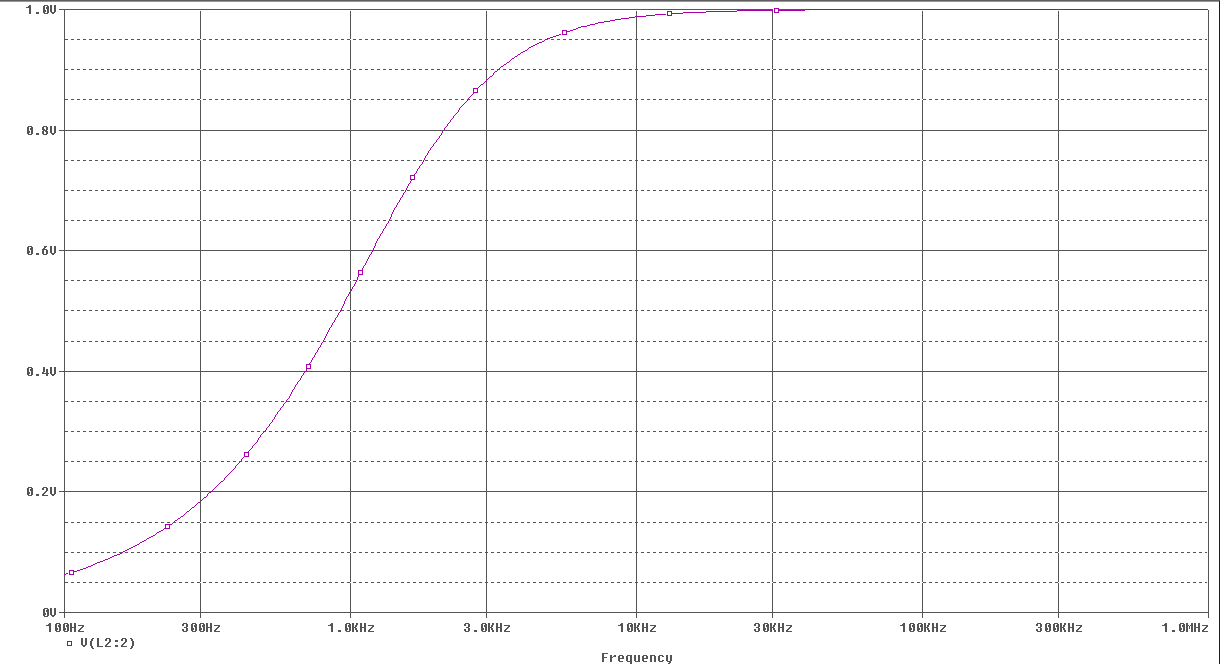
\includegraphics[width=11cm,height=7cm]{Img/Fuente_AC_RL_AC_sweep}
		
		\newpage
		
		\noindent AC Sweep Vpulse\\
		
		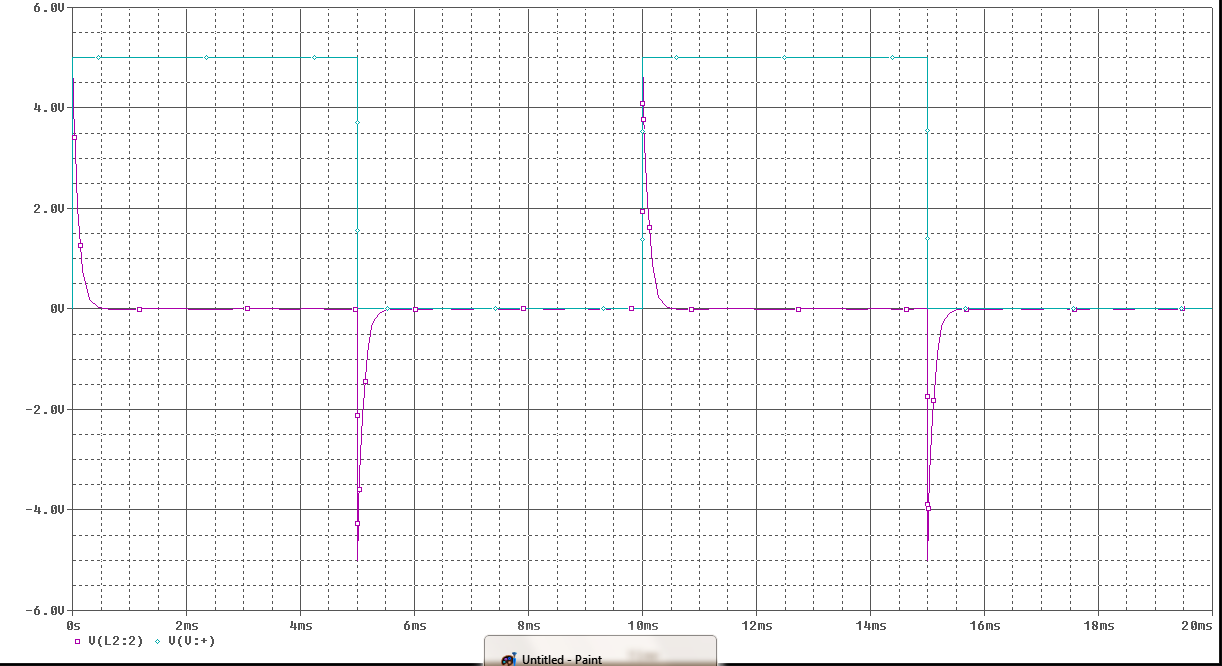
\includegraphics[width=11cm,height=7cm]{Img/Fuente_AC_RL_Vpulse}\\
		
		\item \textbf{Circuito 5}- Corresponde a la figura 2.3\\ 
		
		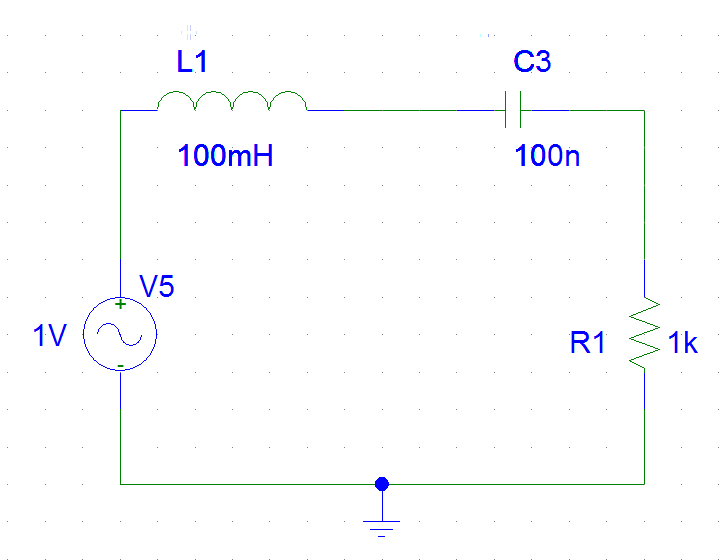
\includegraphics[width=11cm,height=7cm]{Img/ac_rlc}\\
		
		\noindent En este circuito se hicieron cuatro análisis ac sweep, uno sobre la resistencia, sobre la inductancia, sobre la capacitancia y uno sobre la inductancia y la capacitancia en serie. Resultando en:
		
		\newpage
		
		\noindent AC Sweep sobre la resistencia\\
		
		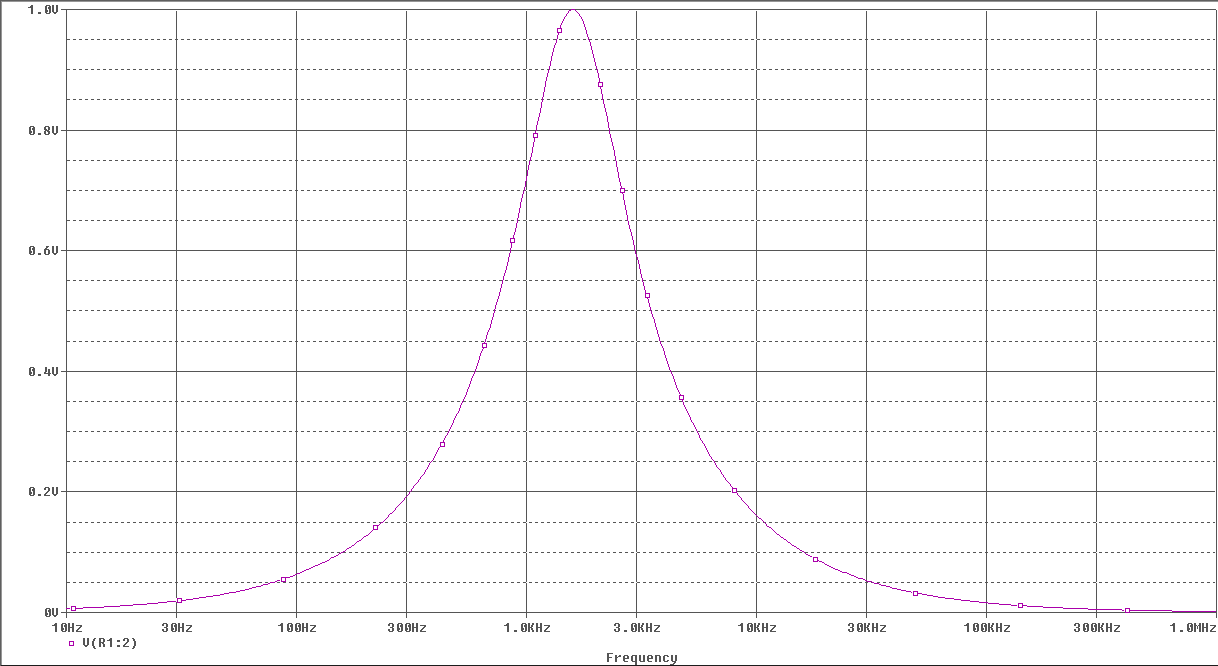
\includegraphics[width=11cm,height=7cm]{Img/Fuente_AC_RLC_AC_Sweep_Resistencia}\\
		
		\noindent AC Sweep sobre la inductancia\\
		
		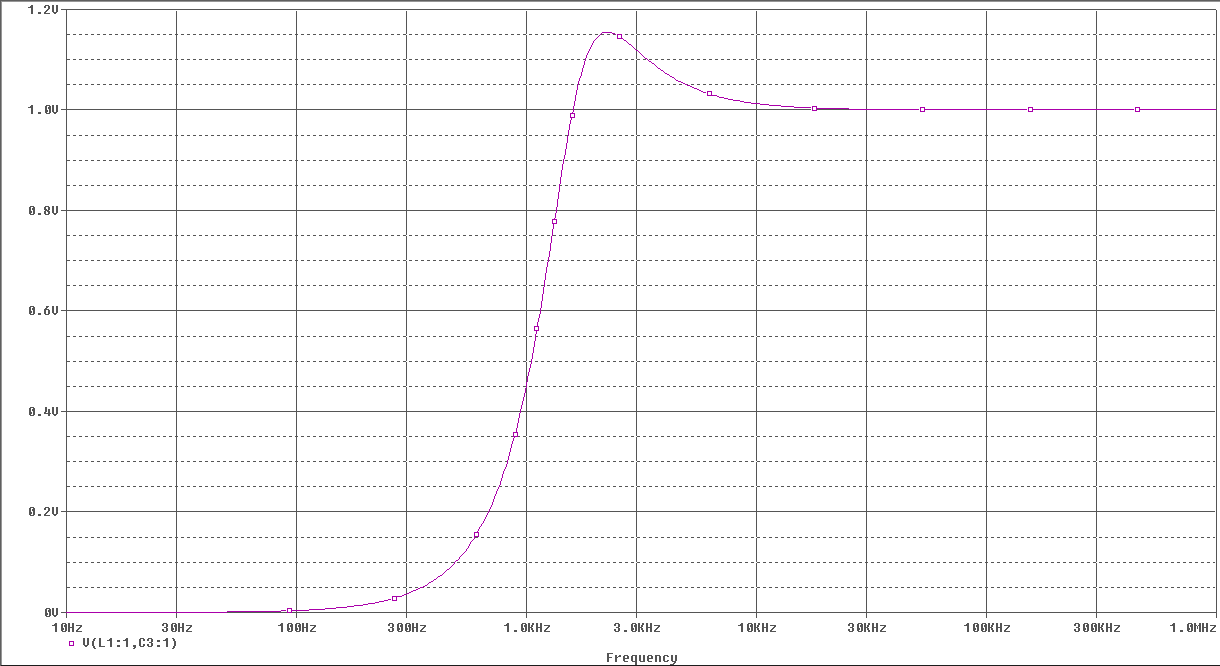
\includegraphics[width=11cm,height=7cm]{Img/Fuente_AC_RLC_AC_Sweep_L}
		
		\newpage
		
		\noindent AC Sweep sobre la capacitancia\\
		
		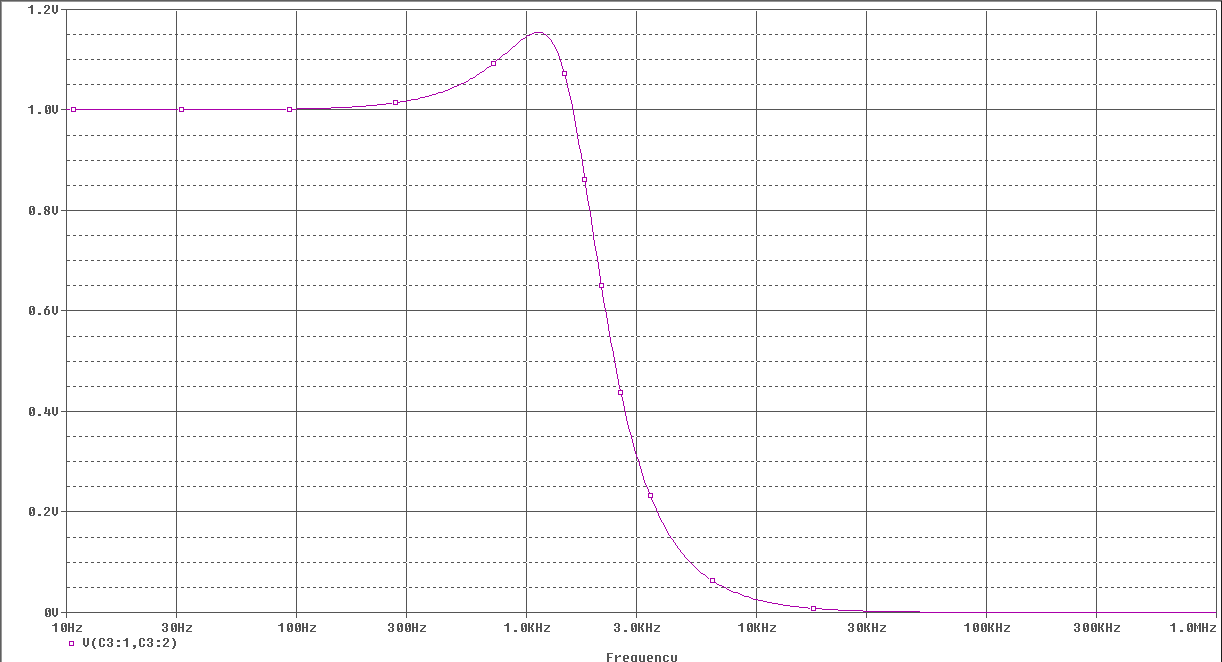
\includegraphics[width=11cm,height=7cm]{Img/Fuente_AC_RLC_AC_Sweep_C}\\
		
		\noindent AC Sweep sobre la inductancia y la capacitancia en serie\\
		
		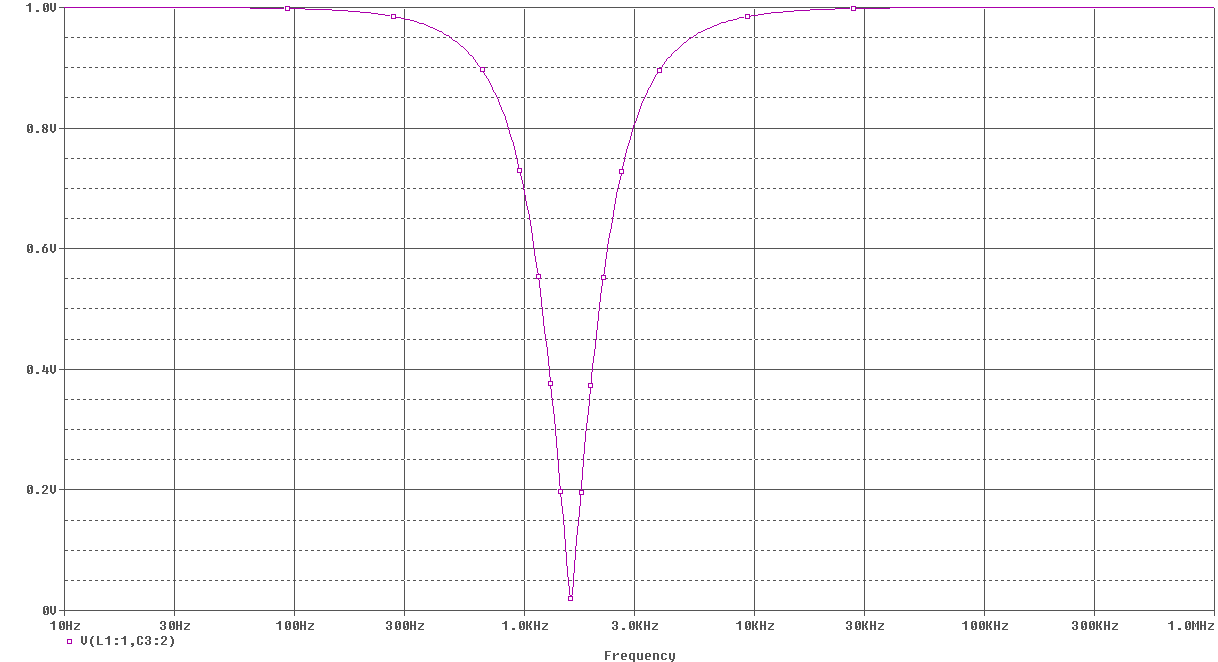
\includegraphics[width=11cm,height=7cm]{Img/Fuente_AC_RLC_AC_Sweep_LC}\\
		
		\item \textbf{Circuito 6}- Corresponde a la figura 2.4 en configuración estrella-estrella\\
		
		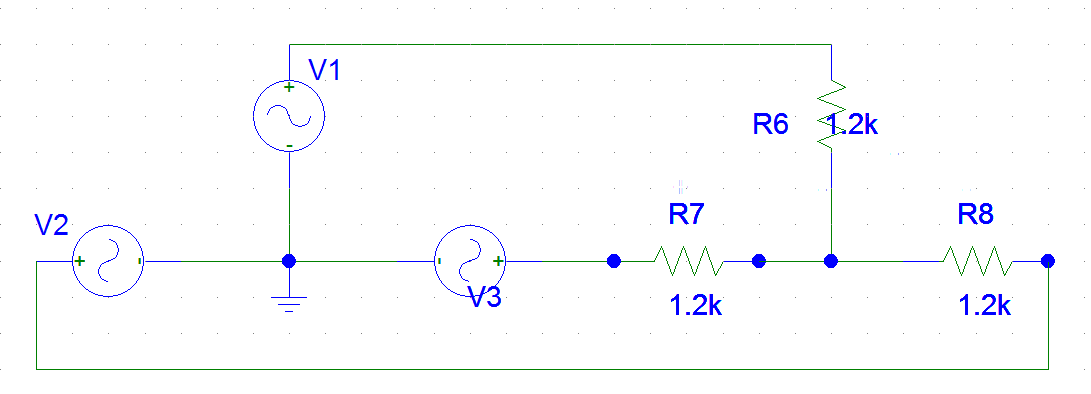
\includegraphics[width=11cm,height=7cm]{Img/trifas_str_str}\\
		
		\noindent Este circuito se sometió a dos análisis transient, uno para las fuentes y otro para las resistencias ambos análisis resultaron en la misma gráfica.\\
		
		\noindent Análisis sobre las fuentes\\
		
		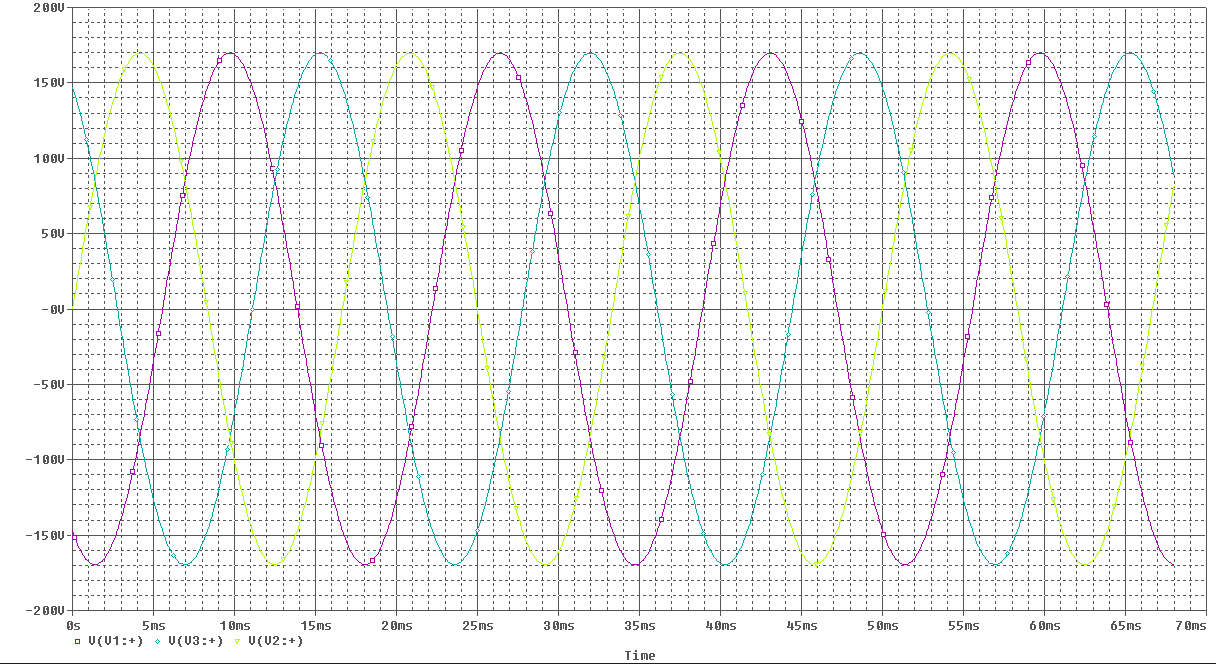
\includegraphics[width=11cm,height=7cm]{Img/Circuito_trifasico_estrella_delta}\\
		
		\noindent Análisis sobre las resistencias\\
		
		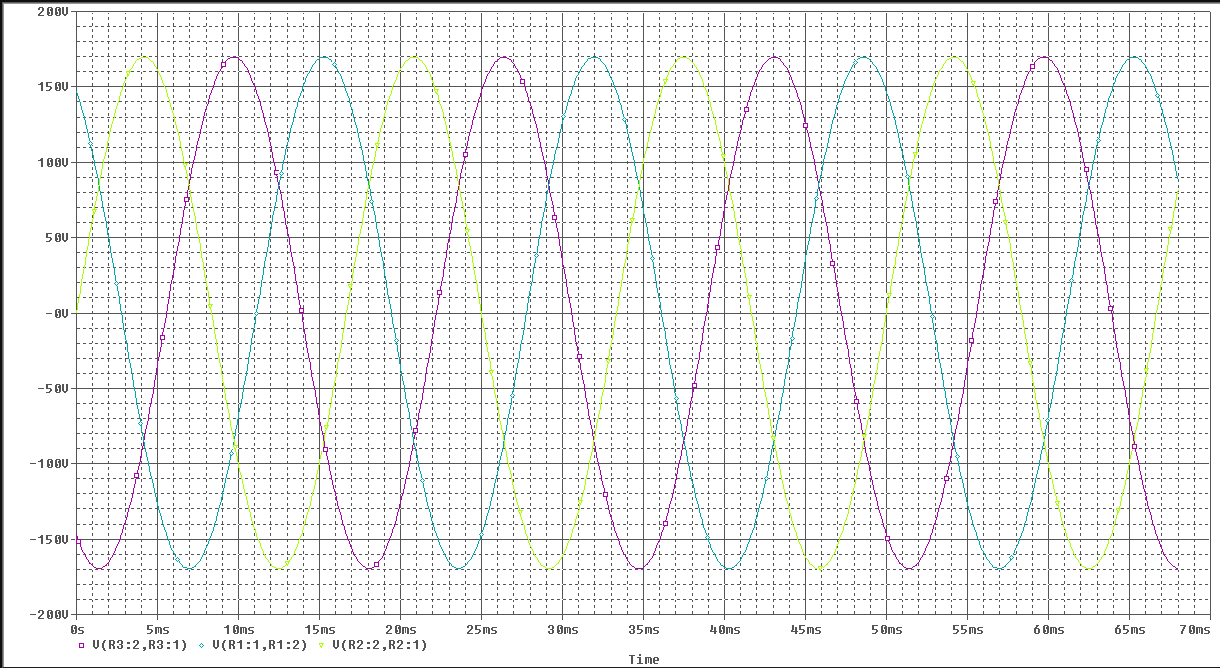
\includegraphics[width=11cm,height=7cm]{Img/circ_trifas_estr_estr_resistencias}\\
		
		\item \textbf{Circuito 7}- Corresponde a la figura 2.4 en configuración estrella-delta\\
		
		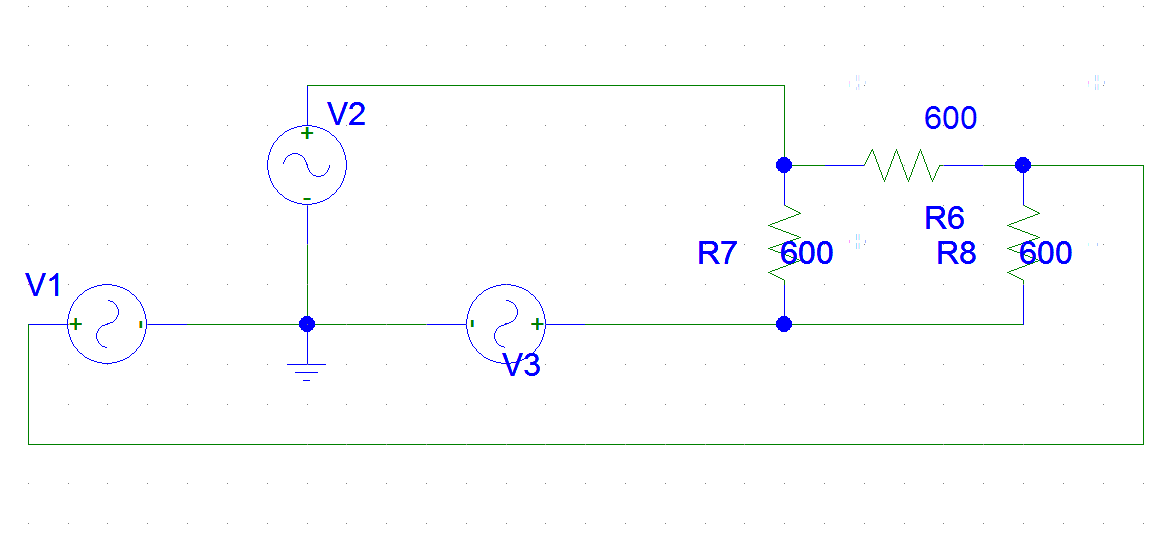
\includegraphics[width=11cm,height=7cm]{Img/trifas_str_dlt}\\
		
		\noindent Sobre esta configuración se aplicó el mismo análisis que en el anterior.\\
		
		\noindent Análisis sobre las fuentes\\
		
		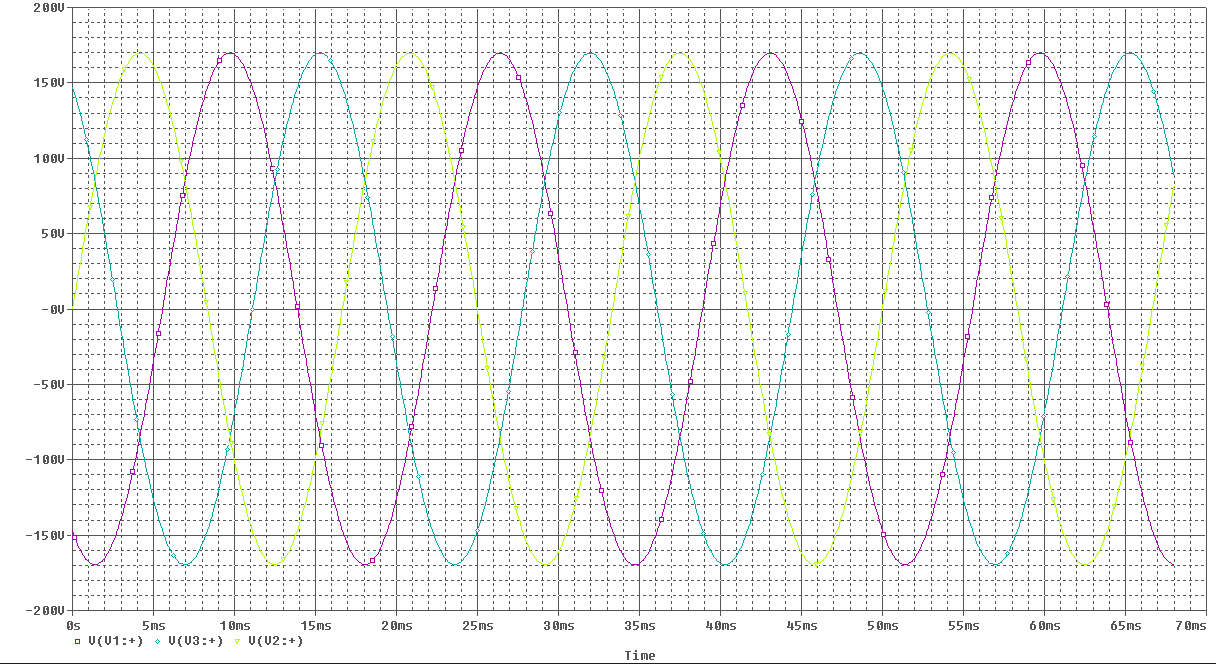
\includegraphics[width=11cm,height=7cm]{Img/Circuito_trifasico_estrella_delta}\\
		
		\noindent Análisis sobre las resistencias\\
		
		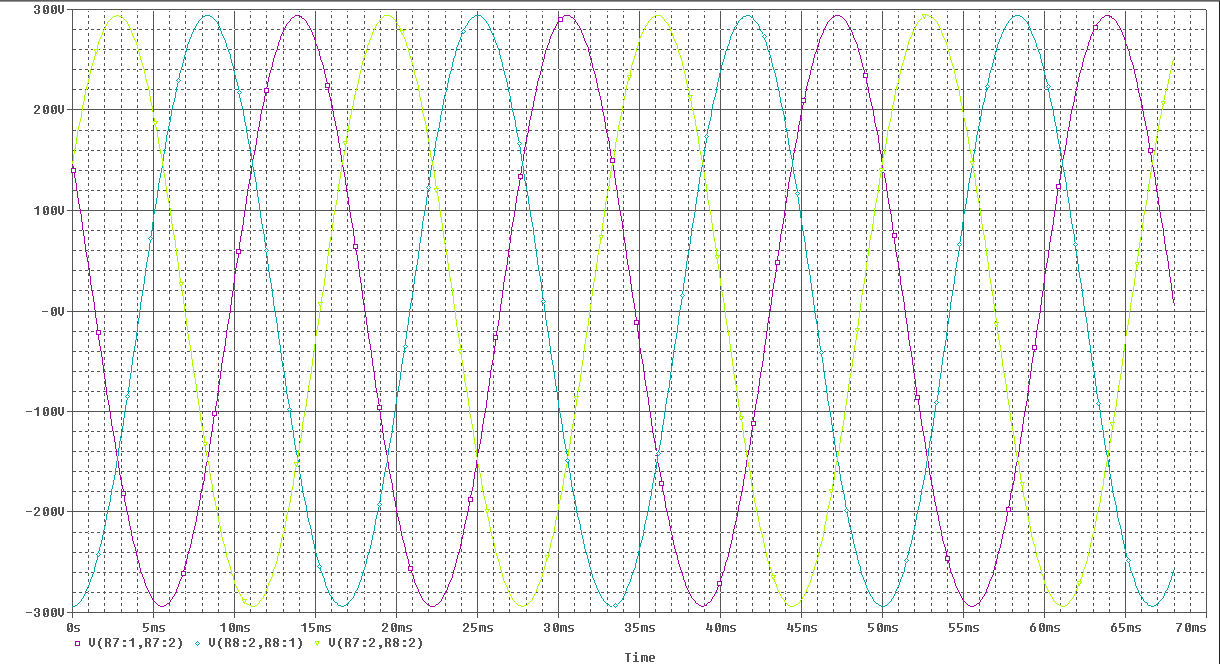
\includegraphics[width=11cm,height=7cm]{Img/Circ_trifas_estr_delta_resist}
		
		\newpage
		
		\item \textbf{Circuito 8}- Corresponde a la figura 2.5\\
		
		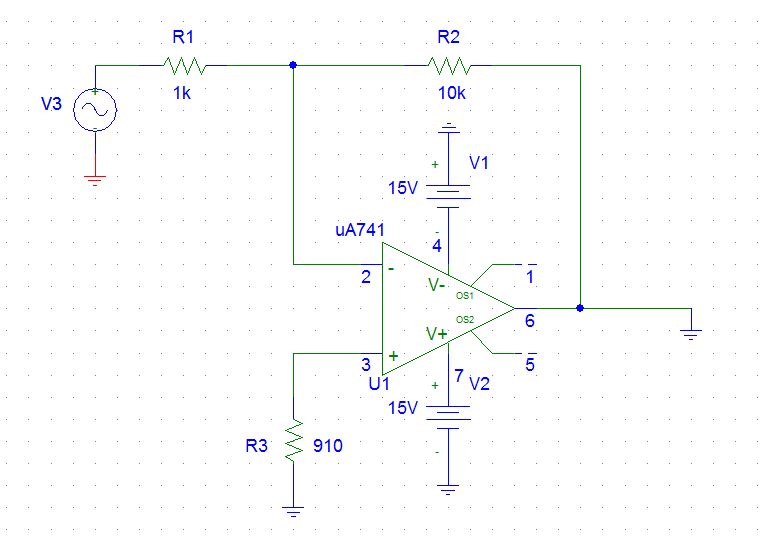
\includegraphics[width=11cm,height=7cm]{Img/opam_ua741}\\

		\noindent En este circuito se realizaron tres configuraciones donde se cambiaba la fuente conectada a $R_1$, en el primero se conectó una fuente constante y se realizó un bias point detail, en el segundo se usó una fuente vsin y se hizo un análisis transient, finalmente en el tercero se usó una fuente vac y se le realizó un análisis ac sweep.\\
		
		\noindent Fuente DC. Análisis Bias Point Detail\\
		
		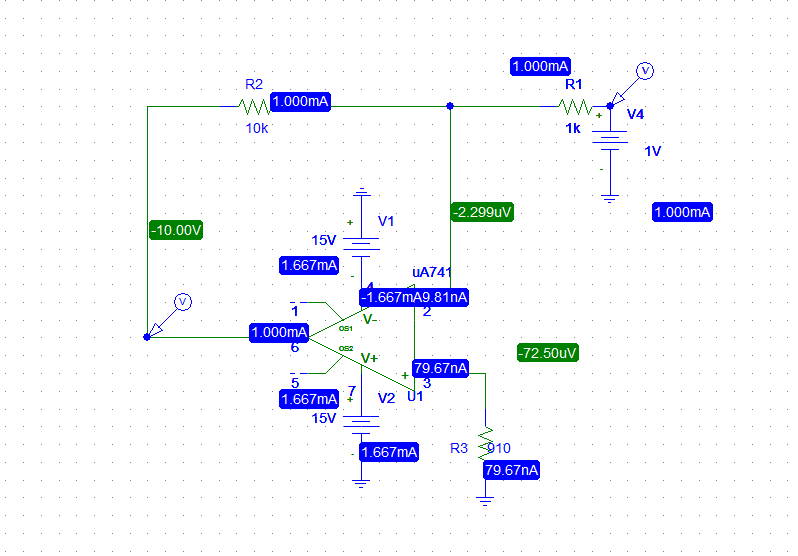
\includegraphics[width=11cm,height=7cm]{Img/opam_ua741_bias_analisis_DC}\\
		
		\newpage
		
		\noindent Fuente AC. Análisis Transient\\
		
		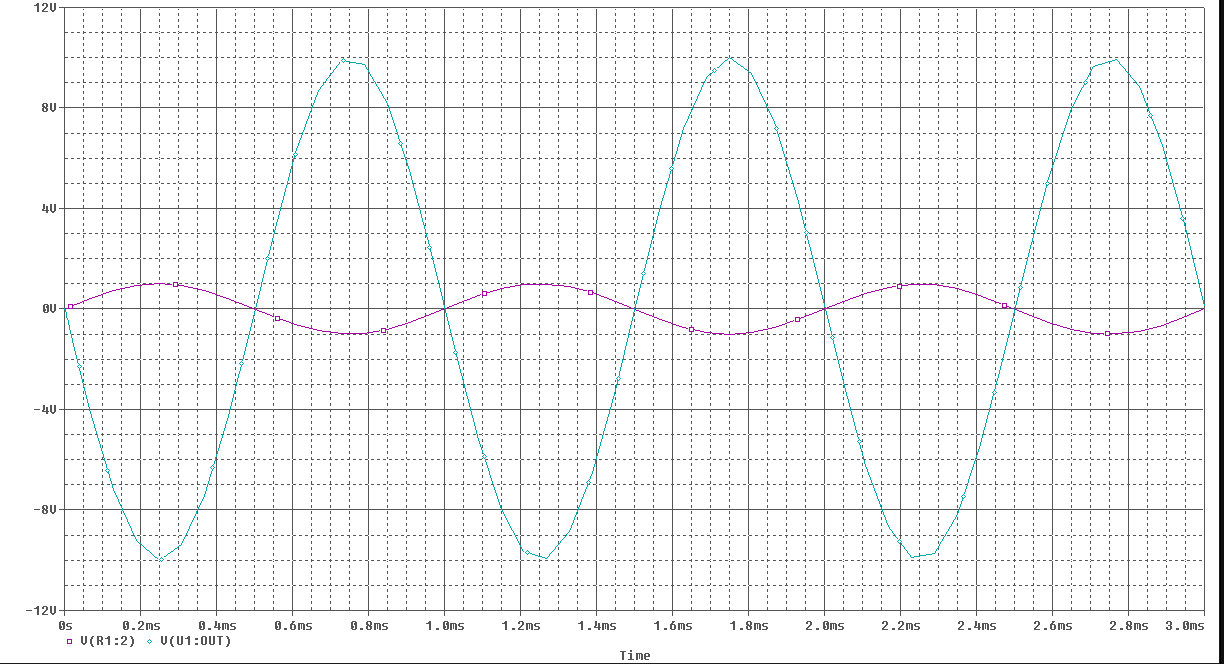
\includegraphics[width=11cm,height=7cm]{Img/opam_ua741_transient_AC}\\
		
		\noindent Fuente AC. Análisis AC Sweep\\
		
		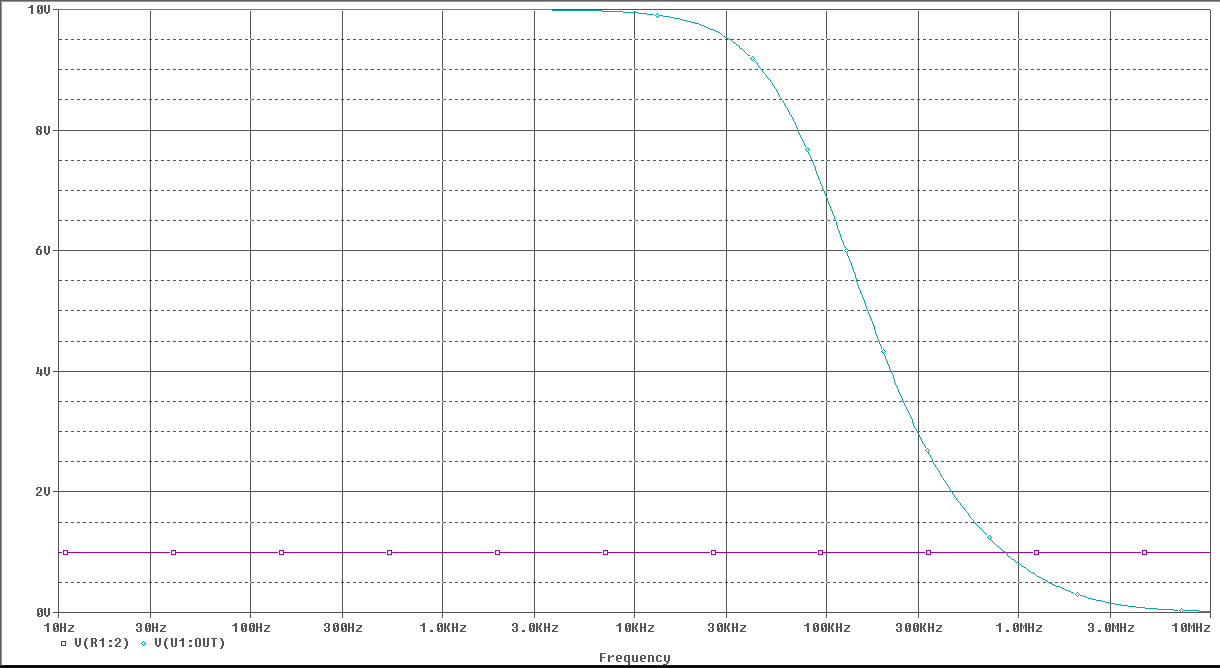
\includegraphics[width=11cm,height=7cm]{Img/opam_ua741_AC_sweep}\\
		
		\newpage
		
		\item \textbf{Circuito 9}- Corresponde a la figura 2.6\\
		
		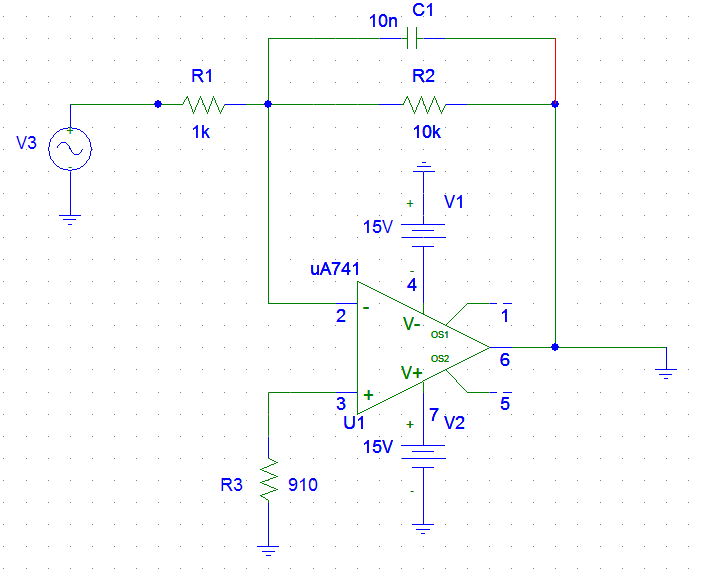
\includegraphics[width=11cm,height=7cm]{Img/opam_ua741_pasa_bajo_act}\\
		
		\noindent Para esta configuración se aplicó un análisis ac sweep que resultó en:\\
		
		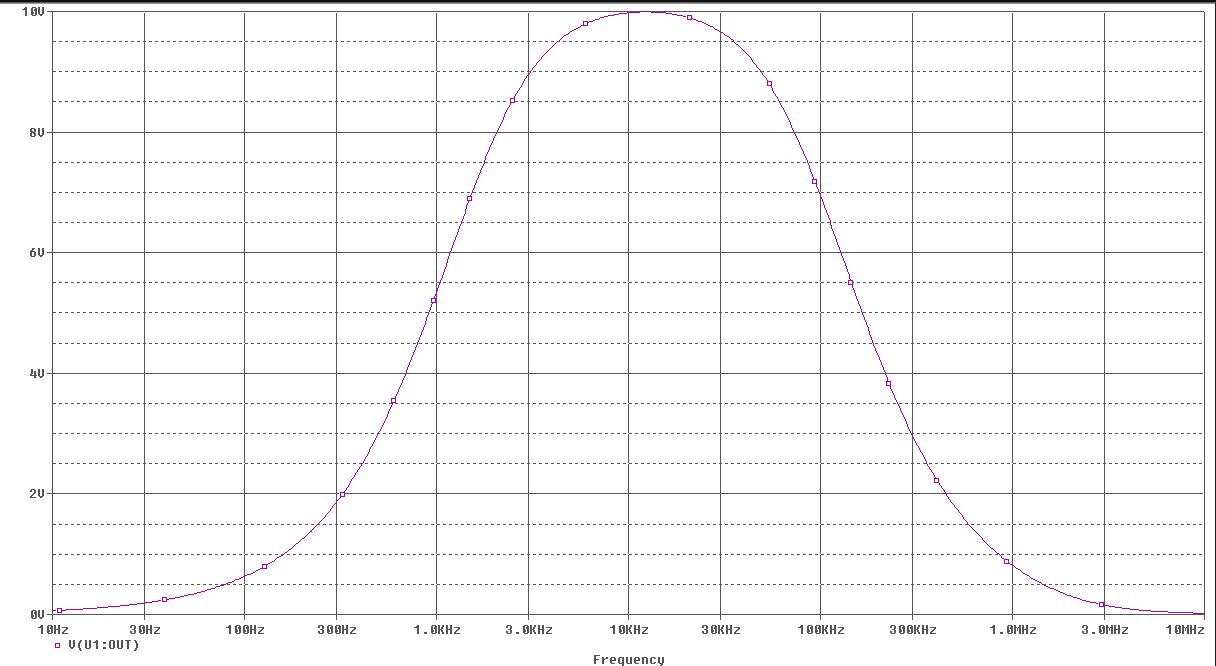
\includegraphics[width=11cm,height=7cm]{Img/filtro_pasa_alto_activo}\\
		
		\newpage
		
		\item \textbf{Circuito 10}- Corresponde a la figura 2.7\\
		
		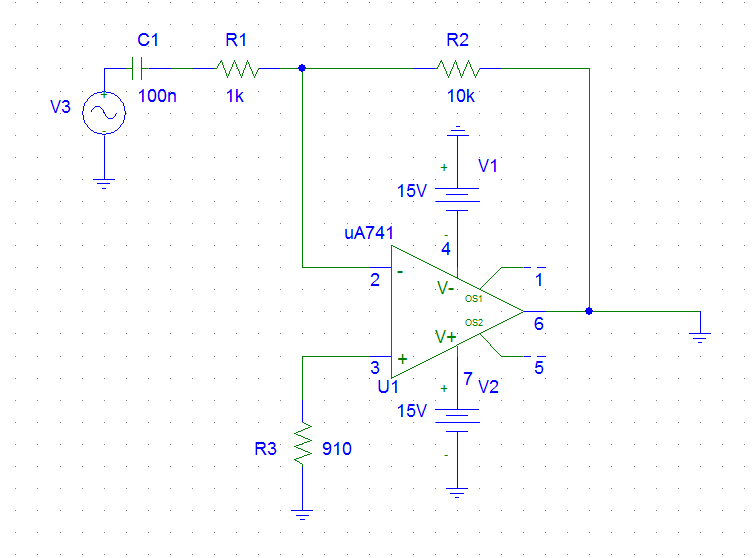
\includegraphics[width=11cm,height=7cm]{Img/opam_ua741_pasa_alto_act}\\
		
		\noindent En este circuito también se implementó un ac sweep:\\
		
		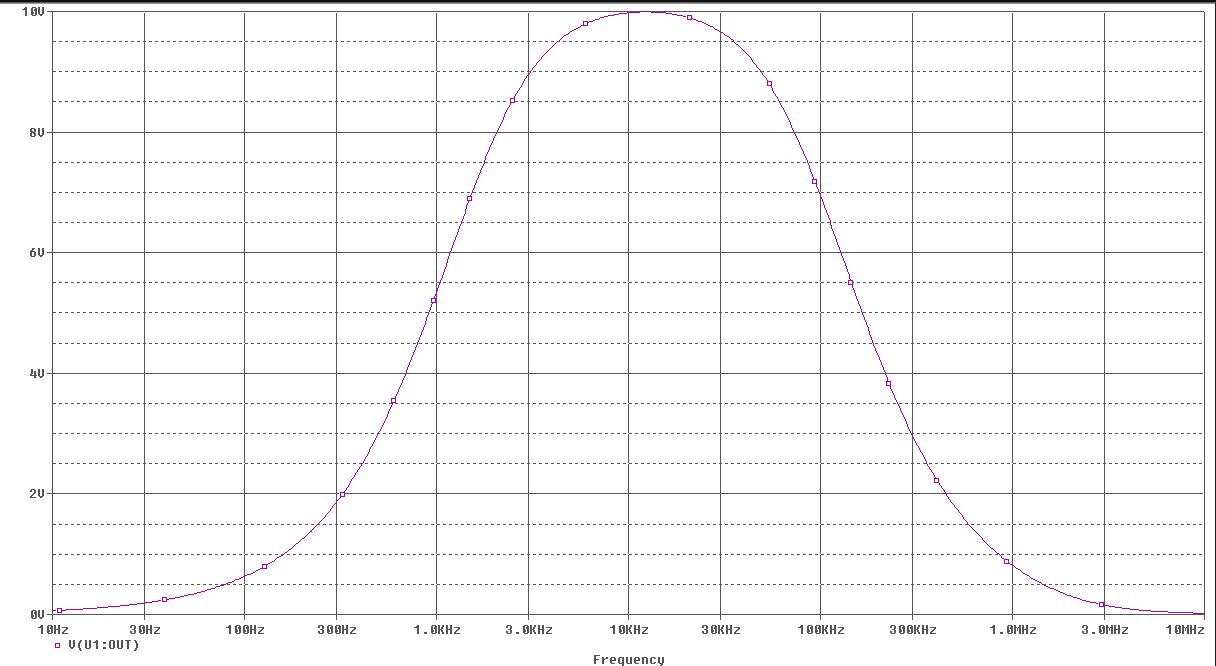
\includegraphics[width=11cm,height=7cm]{Img/filtro_pasa_alto_activo}\\
		
	\end{itemize}
	
	\newpage
	
	\begin{center}
		\textbf{\large ANÁLISIS DE RESULTADOS}\\
	\end{center}
	
	Inserte análisis de resultados
	
	\newpage
	
	\begin{center}
		\textbf{\large CONCLUSIONES}\\
	\end{center}
	
	Inserte conclusiones
	
	\newpage
	
\end{document}